\chapter{Background and Literature Survey}

\section{Java Collection Class}
Java Collection class is a large framework where different data structures like List, Set, Queue, and Map have similar common interface. Except for the Map interface, all the above mentioned data structures are part of the collection class framework. Java also provides an iterable interface through which we can iterate over all these data structures. The collection class provides a lot of common methods for different structures. Some of them are addAll(), copy(), size() etc.


Primary interfaces of java collections are List, Set, Queue, and Iterator. (Map is also considered under collection only). Fig 2.1 shows the class hierarchy of Java Collection classes.

\begin{figure} [h]
    \centering
    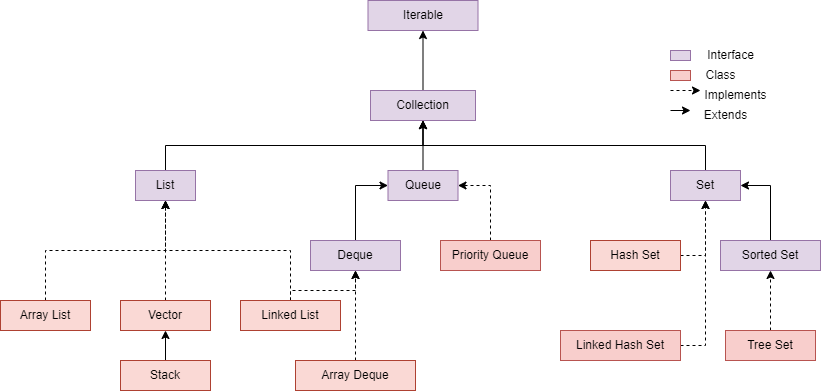
\includegraphics[width = \textwidth]{images/Collections.png}
    \caption{Java Collection Hierarchy}
    \label{fig:my_label}
\end{figure}

\textbf{List}: A list is an ordered collection of elements where we can have the same copies of multiple elements. ArrayList, Vector, and Stack use this List interface for implementation. Linked List implements both List and Deque.

\underline{ArrayList}  is simply a dynamic array. So the size of the list grows as the number of elements in the list grows\\
\underline{Vector} is also similar to ArrayList except vector accesses are synchronized. ArrayList accesses are not synchronized.\\
\underline{LinkedList} is a double linked list implementation that is used for implementing Deque etc.\\
\underline{Stack} is a LIFO (Last In First Out) data structure that is implemented using the Vector Class.
 
\textbf{Queue}: Queue is a data structure that follows FIFO order of elements except for a few cases like Priority Queue and Deque.

\underline{PriorityQueue} is simply an implementation of the heap or we can say the elements come out of the list in the order of their priorities. We can set the priority order by using a comparator function. The default priority is increasing order of the elements.

\underline{Deque} is a double ended queue in which we can insert and delete the elements from both sides. It is implemented using LinkedList Class and ArrayDeque. For normal queues also we will use deque only.

\textbf{Set}: Set is a data structure where there will be no duplicates. It is of two types. One is where there is no order of elements called as "HashSet" and in the other one the elements will be in sorted order (increasing order by default) called "SortedSet".

\underline{HashSet} is implemented using the technique of hashing so that there will be no importance to order.

\underline{SortedSet} is implemented using balanced binary search trees (Red-Black) so that the elements order can be maintained.

We also have \underline{Iterable} interface through which we can iterate over all the elements in any structure mentioned above. Besides this, the Map framework is also considered under Collections only, in which again we have subclass like HashMap, TreeMap, etc.

\section{Soot}
Soot \cite{Sable_McGill} \cite{Soot_2008} is a framework that is used for Analyzing and Optimizing different Applications that use Java. Soot offers a lot of static analysis techniques like call graph construction, intra procedural data flow analysis, use chains, etc. Soot mainly accepts 4 types of codes as inputs. They are Java bytecode, Android Byte Code, Jimple, Jasmin. It can convert the code into four intermediate representations as Baf, Jimple, Shimple and Grimp.

Currently, we use Jimple for analyzing the code because it follows a simple 3 operand Code Representation and also the previous "Followup tool" was written based on Jimple representation only. Jimple only uses 15 types of instructions in the code.

Following are the type of statements in Jimple :
\begin{enumerate} [blt]
    \item Core statements: NopStmt, IdentityStmt, AssignStmt
    \item Intra-procedural control flow statements: IfStmt, GotoStmt, TableSwitchStmt and LookupSwitchStmt
    \item  Inter-procedural control flow statements: InvokeStmt, ReturnStmt, ReturnVoidStmt.
    \item Monitor statements: EnterMonitorStmt and ExitMonitorStmt
    \item ThrowStmt and RetStmt
\end{enumerate}


\section{SPARK}
Soot framework provides Context insensitive built in points to analysis using SPARK. This points to analysis is used to detect the memory location pointed by the pointer while executing the program. This is used in the Followup Tool.

\section{JavaCC and JTB}
JavaCC \cite{JavaCC} is a tool that is used to generate the parsers for different grammars that are written in "JavaCC" format. It accepts the grammar and generate the Java code which can verify the rules that are written according to the defined grammar. JavaCC allows extended BNF specifications like *,?,+. To define Tokens we use general regular expression syntax in Java.

JTB \cite{JTB} is a syntax tree builder which takes a JavaCC format grammar as input and generates "Visitors and another JavaCC grammar file" as output which contains annotations for each node in the syntax tree. Using these annotations we can extract the required elements we want from the rules. Along with the JavaCC grammar file, it also generates Visitor and GJVisitor interfaces which are implemented by DepthFirstVisitor and GJDepthFirst. We can modify these default definitions provided by the methods in the visitors to process different inputs matching the specified grammar.

\section{Followup Tool}
Followup Tool \cite{Vishnu_Kiran} is a tool that is used to get the followup methods of the current function. In this tool, if we give a program and a fully Qualified method name as input then it returns all the follow-up methods of the input method that are referenced by either the calling object of the input method or the objects that are present in the arguments of the input method.

This tool was developed using Soot and SPARK with the help of points to analysis concepts. Currently, this tool takes the benchmark name and the method for which we want to find out the followup functions as command line arguments.The general usage of the Followup Tool is 
\begin{lstlisting}[style = keywords]
java -cp .:soot-4.3.0-jar-with-dependencies.jar followup.Followup_Function_Main {benchmark-name} {method-name} {method-arg-number}
\end{lstlisting}

During the project, we made several extensions to the tool. Firstly, we fixed some bugs. Then, we added the functionality to specify the object for which we want to find the follow-up methods. 